%
% File: chap01.tex
% Author: Liam O'Shea
% Description: Introduction chapter where the boxing goes.
%
\let\textcircled=\pgftextcircled
\chapter{Background \& Research}
\label{chap:intro}

\initial{T}his chapter describes and explains boxing concepts which are important to understanding the goal of the project. It gives an overview of the types of punches a boxer must execute along with common errors associated with those. It also reviews relevant literature in areas covered by this thesis and explores the current cutting edge possibilities. Finally I present an overview of the potential techniques that can be used for my project after analysing a variety of different techniques for their suitability based on the literature review and cutting edge methods.

%=======
\section{Boxing Background}
\label{sec:sec01}
Boxing requires an incredible amount of co-ordination and timing as well as the ability to rapidly execute punches in a controlled and precise manner. Unlike professional boxing which is 12 x 3 minute rounds an amateur bout is 3 x 2 minute rounds which changes the dynamics of the contest. Amateur boxing relies on a points scoring system since there is often insufficient time for knockouts, requiring amateur boxers to rely on the mastery of technique and proper form. For example dropping a guard for a split second can open you up to an experienced boxer and could spell disaster.

As someone who has boxed for over 5 years and captain of the University of Bristol's Amateur Boxing Club (UOBABC) I understand the difficulties of developing good technique and how much time and experience is required from a coach to develop a new boxer. This one-on-one time is incredibly valuable but also expensive and for the large majority very hard to get. ZerotoHero aim is to be able to identify different types of punches and to offer feedback on the quality of the movement. This will bring some much needed expert advice to a beginner who can practice in the comfort of their own home.

I am using my own experience and that of local professionals, coaches and local legend Denis Stinchcombe MBE the centre director of Riverside Youth Project and Registrar for the Western Counties for the Amateur Boxing Association.
 

\subsection{Motivation}
\label{subsec:subsec01}
This research is borne out of a desire to improve access and cost to boxing coaching which are problems I have encountered first hand through the University Boxing Club. In a wider context it could be used in developing countries where physical access to coaches with the required expertise may be difficult as well as local clubs in the UK.
Every year UOBABC takes in new members that are total beginners. We spend an enormous amount of time and effort helping them learn the basics and encourage people to practice at home. The problem from a boxers perspective is that it is incredibly hard to spot your own faults, especially without experience.
If it was possible to practice at home with the benefits of coaching it would bring massive improvements to a trainees ability. The current most effective way to train as an individual is to stand in front of a mirror and observe yourself while shadow boxing.
It could also be used as a way to introduce younger children to the sport since the Kinect is incredibly popular in that demographic and so 
is a good choice from an inclusion perspective.
\section{Boxing Technique}
\label{sec:sec02}
For the scope of this project I am going to focus on the most common orthodox stance. There are tens of slight variations on each punch but I am going to focus on the core foundations and important principles from which these can be built.
\subsection{Stance}
\label{subsec:subsec02}
The most fundamental building block of boxing is the stance, that is how you hold and position your body as well as the placement \& orientation of your feet. A good stance is crucial since it allows the boxer to be well balanced and light on their feet, allowing fast movement in any direction as well as the ability to quickly duck, weave, slip and bob and lay back to avoid punches. It is also crucial for offence since the power from punches come from the transfer of weight from one leg to another which requires a very specific twisting hip movement. Often beginners forget this crucial step and so I'm hoping to use this unique trait to help me judge quality later on. A successful stance should have the following characteristics:

\begin{itemize}
  \item Left foot forward, right foot back with a distance slightly wider than shoulder width with a 45 degree angle twist.
  \item Right heel of the ground at all times with weight distribution mostly on your back leg.
  \item Chin tucked down.
  \item Right hand on the right hand side of your chin, left hand should be a few inches in front of the left side of the face.
  \item Elbows tucked in to protect the torso section.
  \ldots
\end{itemize}

\subsection{Punches}
\label{subsec:subsec03}
\paragraph{Jab}
The elbow should stay tucked in while the left fist extends with palms facing inwards before twisting your wrist at the last moment. The natural thing to do is extend the punch with palms facing down, unfortunately this immediately makes the elbow stick out which allows the opponent to easily see you are about to throw a punch (telegraphing) while opening up your body for a counter attack. The punch should also finish so your arm is fully extended which helps to extend your reach and protect your chin before speedily returning it to the guard position.\newline
Target Characteristic: Elbow movement

\paragraph{Cross}
The cross is designed as your heavy straight punch and as such is slower but more powerful. To get a snappy and powerful punch it is important to transfer your weight rapidly from your back leg to your front leg, twisting your hips.\newline Target Characteristic: Twisting of the hip\newline
Target Characteristic: Distribution of weight to the front foot


\paragraph{Hooks}
Your elbow should be raised to shoulder height and your fist and shoulder should be at 90 degrees to each other. A transfer of weight between the front foot and back with the twisting of the hip is essential.\newline
Target Characteristic: Elbow being raised to parallel\newline
Target Characteristic: Hip twist resulting in weight transfer from front to back\newline

\paragraph{Uppercuts}
This required the fighter to crouch down into the squat position and throw a punch vertically upwards, with the aim of striking the opponent's chin.
Target Characteristic: Sufficient crouching before releasing the punch\newline
Target Characteristic: Directly vertical punch, keeping guard close at all times.\newline

\section{Kinect}
This section provides some background information about Microsoft Kinect that is important for understanding the features and limitations of Kinect Analysis. According to Microsoft, the Kinect  has worldwide sales of approximately 28 million units and contains an RGB camera, an infrared (IR) emitter and an IR depth sensor as well as a multi-array microphone. The interaction space of the Kinect is limited by the field of view of the Kinect cameras. The Kinect has a 43\degree vertical by 57\degree horizontal field of view. The Kinect sensor can be tilted using a built-in tilt motor. Tilting the Kinect increases the interaction space by $+27$ and $-27$ degrees.
The Kinect sensor provides sensor data in form of data streams. It can capture audio, color and depth data. In addition, it can process the depth data to generate skeleton data. Therefore, the Kinect offers four different data streams that can be accessed: audio stream, colour stream, depth stream and skeleton stream. The streams can deliver at most 30 frames per second (FPS) using a resolution of $640\times480$ which drops to 12 FPS with a resolution of $1280\times960$.

\begin{figure}[h]
\centering
\begin{minipage}{7.0cm}
    \centering
    \subtop[]{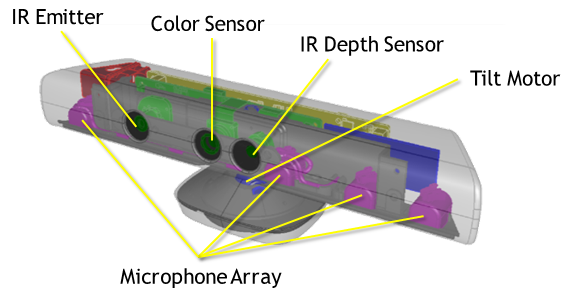
\includegraphics[height=0.15\textheight]{fig02/kinect}}
    \label{fig:1}
\end{minipage}
\begin{minipage}{7.0cm}
    \centering
    \subtop[]{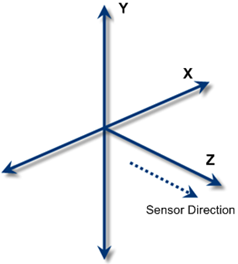
\includegraphics[height=0.15\textheight]{fig02/xyz}}
    \label{fig:2}
\end{minipage}
\mycaption[ALLData] {(a) Kinect 
(b) Kinect Dimensions}
\end{figure}


\begin{figure}[h]
    \centering
    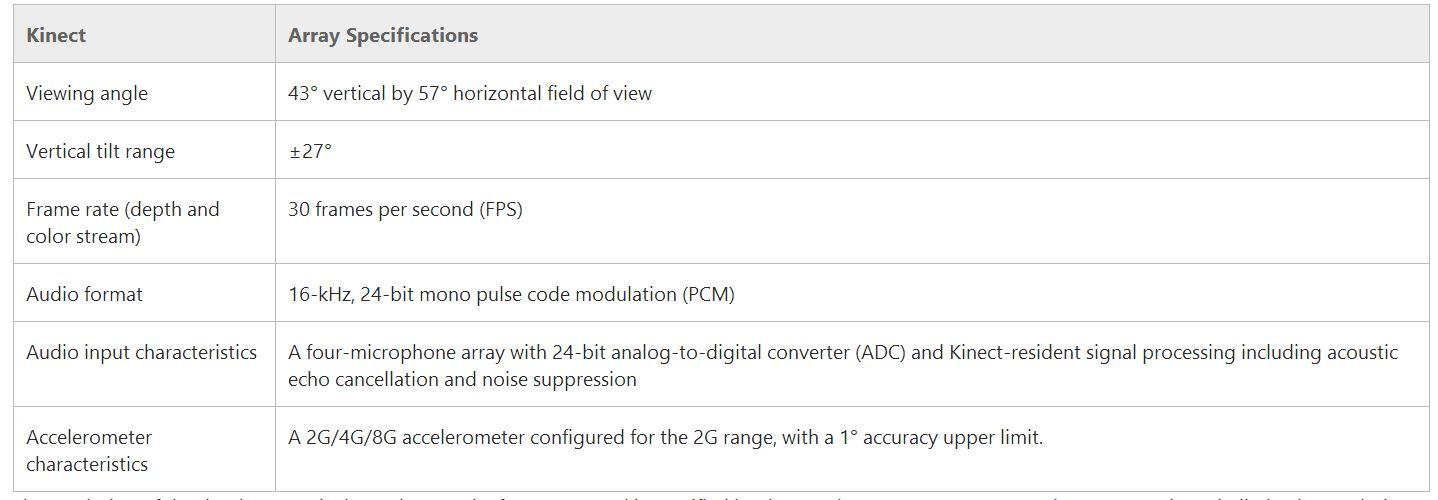
\includegraphics[height=0.25\textheight]{fig02/kinspecs.jpg}
    \mycaption[Kin Specs]{Kinect Specifications}
    \label{fig:kinect}
\end{figure}
\begin{figure}[h]
    \centering
    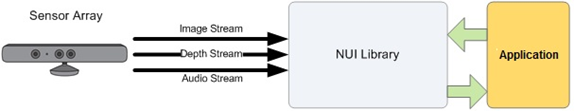
\includegraphics[height=0.15\textheight]{fig02/pipeline}
    \mycaption[Kin Specs]{Kinect Specifications}
    \label{fig:kinect}
\end{figure}

\paragraph{Depth \& Infrared Stream}
The depth sensor generates invisible IR light to determine an object's depth from the sensor. The primary use for the IR stream is to improve external camera calibration using a test pattern observed from both the RGB and IR camera to more accurately determine how to map coordinates from one camera space to another. \cite{irstream} The NUI API uses the depth stream to detect the presence of humans in front of the sensor.\cite{winSDK} Skeletal tracking is optimized to recognize users facing the Kinect, so sideways poses provide some challenges because parts of the body are not visible to the sensor.

\begin{figure}[h]
    \centering
    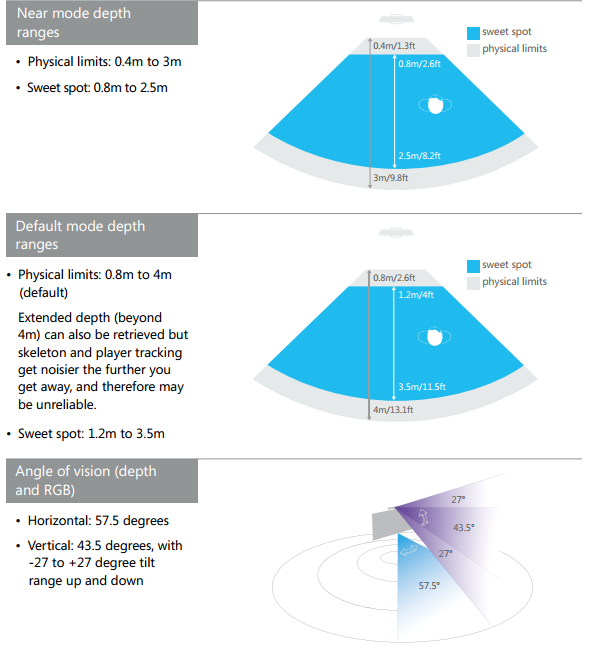
\includegraphics[height=0.45\textheight]{fig02/kinDepth}
    \mycaption[Kinect Depth Specifications]{Kinect Depth Specifications.}
    \label{fig:kinsdepth}
\end{figure}


\subsection{Skeleton \& Joint Tracking}
The Kinects default tracking mode can track up to 20 joints per skeleton providing the subject is standing relatively face on and are fully visible to the sensor. Although the Kinect is capable of different modes (e.g. sitting) this is not relevant in the context of my project.
Each skeleton frame contains the position of each joint as well as information about the tracking quality. Joints can have one of three different tracking states,  Not Tracked (0), Inferred (1) and Tracked (2), this flag is useful as an indicator of the quality of the measurements you are receiving for a particular joint. When possible, tracked joints are used to help calculate the position of those joints that cannot be directly tracked hence the ability to infer joints. The Kinects default tracking mode is designed to track people who are standing and fully visible to the sensor. The default range requires skeletons to be at least 80 centimetres away from the device to be tracked properly.

\begin{figure}[h]
    \centering
    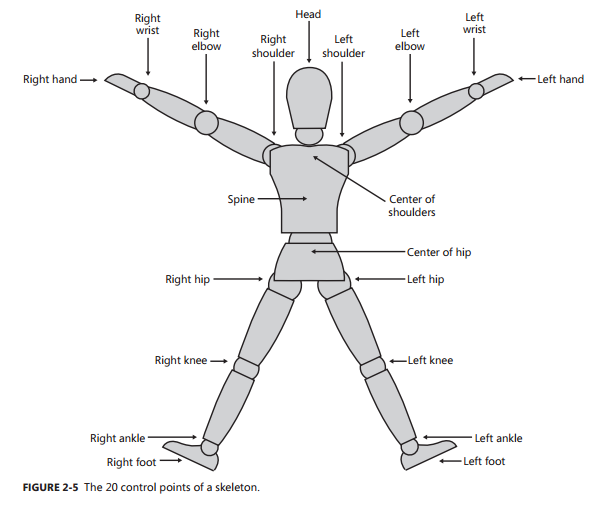
\includegraphics[height=0.40\textheight]{fig02/kinSkel}
    \mycaption[Kinect Joint Tracking Skeleton]{Kinect Joint Tracking Skeleton.}
    \label{fig:kinskel}
\end{figure}



\section{Literature Review}
The Kinect is currently a rich area of research in its own right and it straddles the fields of Image Processing and Computer Vision as well as Human computer Interaction which are exciting and popular areas of research. Recognising punches is an example of activity recognition in which there has been a fairly large body of work using the Kinect since it was released to PC in 2012 by Microsoft.

With the development of such a low cost device researchers have shifted their focus onto action analysis and gesture recognition based on depth maps. I wanted to see what was capable with the Kinect at the cutting edge of research so I consulted the most recent papers from the conference on Computer Vision and Pattern Recognition (CVPR), International Conference on Computer Vision (ICCV) \& European Conference on Computer Vision (ECCV) as well as an array of other resources to find the most relevant and useful research. 

Examples of current work are a customisable hand gesture recognition interface \cite{chr}, physical therapy instruction \cite{physio}\cite{Kinect2012}, Karate instruction \cite{karate} and quality assessment of the reach and grasp of stroke survivors \cite{rehab}.

Oya caliktutan developed a graph-based method for aligning two dynamic skeleton sequences with the aim of action recognition and `objective quantification of goodness' of said action. \cite{Celiktutan2013a} Depth maps are used similarly to the real-time skeleton tracking algorithm developed by Shotton. \cite{Shotton2011}


In 2013 a controlled study of 16 people who were blind or who had low vision was ran to test the usefulness of Eyes-Free Yoga: An Exergame Using Depth Cameras for Blind \& Low Vision Exercise. The purpose of this was to teach the participants yoga poses using audio feedback and a positive response from participants.\cite{Rector2013} The study took the Kinect joint positions and calculated joint angles while using heuristics for each pose. However the study only measured success using 6 unique static poses that were required to be held for an extended period of time. In contrast boxing requires fast repeated movements with many of the movements sharing similarities which make them harder to differentiate. Therefore I did not find this useful for evaluation the feasibility of my project.

The Kinect has also been used to evaluate salsa dancers performance with comparison to a professional dancer in real-time\cite{Alexiadis2011}\cite{vdpe}. A score was achieved by adding three different metrics, one from the correlation coefficient of quaternions, another using joint velocities and finally a `'3D flow Error,'' calculated from frame vectors. Quaternoin correlation was then used to estimate the time-shift between two dancing sequences.\newline
The experimental results were encouraging with most of the scores consistent with real-life rankings with the exception of a few poor results due to bad skeleton calibration and tracking. This work draws strong parallels in what I am trying to achieve and demonstrated that the Kinect was a viable option for my work.

Work on disc throwing performance\cite{Yamaoka2013} also showed some promise with limited success with the lower ability groups improving their movement. This approach simply used joint angles to measure 5 different phrases of the throw and compare that to joint angle rules. I found this to be overly simplistic in comparison to the project I am trying to achieve although it did indicate that joint angles may be a useful technique for judging movements.

Xia took each joint position and represented this using a histogram. \cite{hmm1} The joint positions were converted from Cartesian co-ordinates to spherical co-ordinates and splitting the sphere into several grids. A sequence of poses was recorded and represented as histograms before using Hidden Markov Models for classification.  Some of the concepts used in this work were adapted from Li \cite{3dbag} in particular the `bag of 3D points' used to characterise poses.

Previous implementations have used joint weighting which have been shown to increase recognition performance with weighted dynamic warping\cite{dtw1} and decision forests \cite{randforest}. Join weighting is also used with a newly proposed skeletal representation `Sequence of most informative joints (SMIJ)' where at each time instance the most informative skeletal joints are selected depending on the action being taken \cite{SMIJ}. In this work each sequence was divided into small temporal sequence (frames), taking into account joints with maximum variance and represented these `most informative joints' with a histogram for action recognition.

Raptis proposed a different skeleton representation which was designed for `recognition robustness under noisy data'\cite{Raptis2011a} alongside a cascaded correlation-based classifier and a distance metric produced by dynamic time warping  that will match the performed gesture to the closest matching gesture.\cite{Kaewplee}
PCA is applied on only the torso joint and used to estimate the orientation of the skeleton which allows specific relevant features to be extracted.


The most recent research in real-time action recognition methods have been built on random decision forests.\cite{randforest} \cite{Miranda2014} Miranda's 2012 paper\cite{Miranda2012}  and Raptis's paper \cite{Raptis2011a} both use SVM's to identify key poses before passing them to the forest to classify. A comparative summary of `model-based method for body pose estimation and tracking'\cite{Manjuatha2014} show SVM to be a popular and effective technique used in 2013.


 \paragraph{auto seg}
 Using RBB video I have encountered very few methods for automatic action quality assessment although a few approaches have been proposed based on skeleton tracking. 
For example Bianco and Tisato recognize Karate moves based on skeletal joints.\cite{karate}

For each strike a triplet of joints are manually selected and can then be represented by the angles of the joints. K-means clustering is used to obtain a set of key poses and Dynamic Time Warping attempts to align sequences of poses. The distance measure from DTW is then used as a performance evaluation. However the quality of this paper did not seem to me to meet the same standards as many of the others reviewed and the poses used were very static and very different to each other.
Given this I would expect a good classification performance since there should not be too many common features. Since boxing has a much more `closed' guard and the punches share many similarities I am not convinced that k-means clustering will produce good results.


\section{Existing Products}
\par{UFC Personal Trainer}
The closest commercial product is `UFC Personal Trainer' a very broad commercial Xbox game aimed at introducing people to UFC. After evaluating this product it became clear to me that it’s main focus is  exercise regimes rather than technical fighting. Therefore it does not offer the preciseness or technical fighting focus that I require. In this game you technically wrong punches will still register and several movements are unrealistic.

\paragraph{Kinect sports boxing game}
This game has very poor punch discrimination and does not require any sort of real boxing ability. The goal here is usually to punch towards the Kinect controller as quickly as possible. It fails to recognise properly thrown hooks and uppercuts and translate those into the game. 

\paragraph{Fighers Uncaged}
This game has generally poor reviews from reviewers, with most complaints involving the reliability of the Kinect to accurately measure fighting moves. \cite{gamerev1} `'When the fights actually start, pulling off moves becomes a series of desperate flails, trying to get the game to recognize your actions.''\cite{gamerev2} 
and `'The game fails to register most of the movements'', `'The idea was great for Kinect, but something went horribly wrong along the way. Kinect is supposed to register your every kick and punch, but it only catches about the half of them.'', `'the Kinect control is lazily implemented.''\cite{gamerev3} \newline

\paragraph{Literature \& Product Conclusion}
From my research and product comparisons I concluded that the Kinect was a viable option for my project and worth pursing. Crucially however there has been no research specifically into the area of boxing with the Kinect which brings it's own unique challenges. Boxers are trained to be fast, well guarded and to give very little away in their movements, especially punches. Therefore many of the punches and poses are very similar since the goal is to be naturally evasive. This will make segmenting punches and giving useful quality metrics challenging in it's own way unlike say a discus throw. A boxers stance is often quite `closed' so I anticipate challenges tracking obscured joints and the overall accuracy of inferred joint positions. However I could see from the above studies that hip movement could be effectively tracked which was my main concern when evaluating the Kinect since all boxing moves rely on the hip rotation.
\newline\newline 
It is clear that this will not be an easy project. Many years of Microsoft research have gone into the current Kinect but surprisingly games for their flagship console fail to provide tracking accuracy that satisfies consumers. Furthermore no commercial products exist that incorporates proper boxing technique into a game, suggesting there may be limitations with the hardware that prevent this or that it it simple difficult to do. However the research in this area has shown sufficient promise for me to combine my boxing and computer science knowledge to work on this problem.\clearpage
%=========================================================

\section{Dimensionality}
\paragraph{Curse of Dimensionality}
The curse of dimensionality, first discussed by Richard E Bellman in his book Dynamic Programming\cite{dynprog} is the term for a set of problems that occur when using high dimensionality data. As dimensionality increases as does the search space, resulting in the available data become sparse. In order to obtain accurate, reliable and statistically sound results the total amount of data required can grow exponentially in relation to the dimensionality. Likewise the organisation and searching of non-reduced data becomes difficult, with space and search time dependent on data volume. Searching and organising data also relies on the ability to group instances into groups that share similar characteristics, unfortunately if the data appears to be dissimilar due to sparseness it can prevent grouping strategies.

Algorithms that can successfully deal with high dimensionality data typically will have high time complexity and {\bf will not always} produce more accurate results than algorithms that work on the lower dimensionality data. Therefore it is sensible to look at some dimensionality reduction techniques which {\bf might}produce better results.

Furthermore since the long-term goal is to give feedback with live data, speed is of the essence. Therefore dimensionality reduction is an important component required to decrease the processing time on any input.

\subsection{Dimensionality Reduction}
Dimensionality Reduction is the process of reducing the number of variables under consideration for any given problem. For example each frame from the Kinect is represented by 80 data points, 60 of which are the x,y,z co-ordinates of the 20 skeleton joints. Considering the Kinect is capable of 30 FPS that is $1800$ data points per second of movement. With long sequences of recordings this could become a huge amount of data to process, most of which could be represented in a reduced dimensionality.

\subsection{Principal Component Analysis (PCA)}
\label{subsec:subsec01}
Principal Component Analysis is a statistical procedure that transforms a set of observations of potentially correlated variables into a set of linearly uncorrelated variables called principal components. The number of principal components should always be less than or equal to the number of original values with the first principal component having the largest possible variance. Each following component will attempt to represent as much variance in the data as possible. In my case I will be looking to reduce my 60 data points per frame into a low dimensionality set that will help me to uniquely identify punches.

\paragraph{Eigenvectors \& Eigenvalues}
The eigenvector of a matrix $M$ is a vector $V$ such that $M\times V$ yields a constant multiple of $V$, the multiplier of which is denoted by $\lambda.$
$$Av = \lambda v$$
$\lambda$ is known as the eigenvalue of $M$ which corresponds to $v$. Any multiple of an eigenvector will have the same eigenvalue as as original eigenvector.

The principal components produced by PCA correspond to the principal eigenvectors of the covariance matrix which are calculated by eigenvalue decomposition. The principal eigenvectors are those with the highest eigenvalues and so are easily deduced. 

\paragraph{Covariance Matrix \& Optimisations }
\begin{wrapfigure}{R}{0.20\textwidth}
\vspace{-15pt}
\hspace{15pt}
\bf{X = } $\begin{bmatrix} X_i\\.\\.\\X_n \end{bmatrix}$\newline
\end{wrapfigure}
If the data is represented in a column vector each with a finite variance then the covariance matrix $\mathbf{\sum}$ is the matrix whose (i,j) entry is the covariance
$$\mathbf{\sum_{ij}} = COV(X_i,X_j) = \mathbf{E}[(X_i - \mu_i )(X_j - \mu_j )]$$
Where:
$$\mu_i = E(X_i)$$ and $$\mu_j = E(X_j)$$
The is equivalent to $$\mathbf{\sum} = E[(X-E[X])(X-E[X])^T]$$ 
with $\frac{1} {n-1}$ added to make the estimate unbiased.

The number of data points in each frame is 60 and the Kinect is capable of 30 FPS which over 120 seconds produces 216,000 data points to represent that sequence. A matrix of this size is costly and slow to find eigenvectors for. Let us say that 60n is the number of data points for frame and m is the number of frames. Take X as size (d x 60n) and $X^T$ as (60n x d) meaning $X^TX$ is of size (60n x 60n), while $XX^T$ is of size (d x d). It is however known that the eigenvalues for $X^TX$ are the same as for $XX^T$ which is useful since this is of a much smaller size and hence less costly.\cite{fastPCA}
The eigenvectors ($v_i$) of $X^TX$ are related to the eigenvectors ($U_i$) of $XX^T$ by the equation $$V_i = X^TU_i$$ with $V_i$ needing to be normalised afterwards. This method can reduce the eigenvalues and eigenvectors produced from a maximum possible $N^2$ for $X^TX$ to M values for $X^TX$.

The M eigenvalues of $XX^T$ will be identical to the first M largest eigenvalues from $X^TX$. This is an important performance step since the goal of my system is to run in real time and this will reduce the time taken.

\begin{figure}[h]
    \centering
    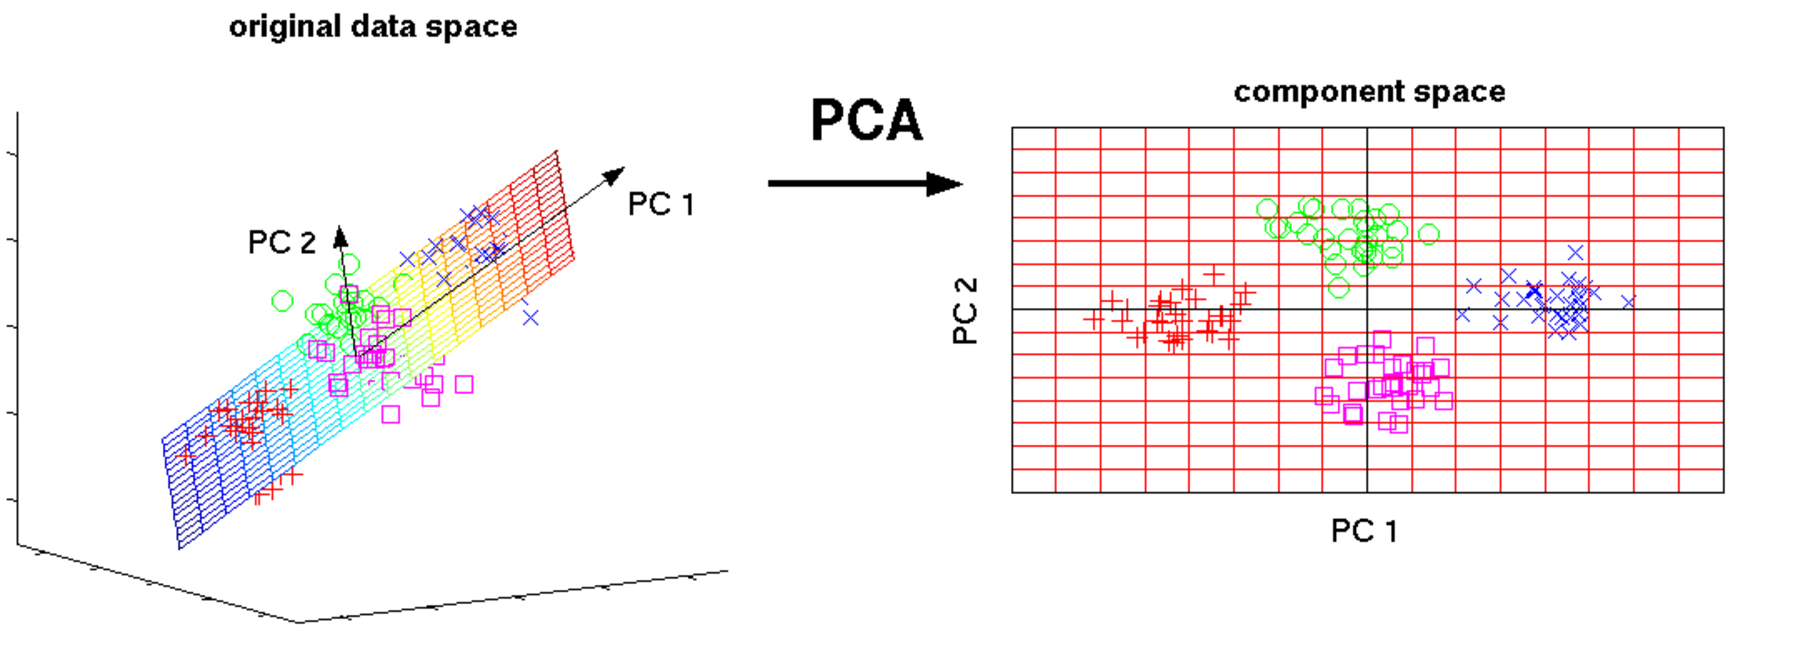
\includegraphics[height=0.25\textheight]{fig02/PCA.pdf}
    \mycaption[PCA Example]{PCA example showing the 1st and 2nd largest eigenvalues and the component space}
    \label{fig:kinect}
\end{figure}


\section{Manifold Learning}
Manifold learning is a Non-Linear Dimensionality Reduction process that transforms high dimensionality data that typically requires multiple dimension to represent it which is difficult to interpret. To simplify the data it is possible to assume that the date lies on an embedded non-linear manifold within the high-dimensionality space. Assuming the manifold has low enough dimensions it can then be visualised in this lower-dimensionality space.

\subsection{Diffusion Maps}
Diffusion maps are a non-linear and relatively new technique developed in $2006$ by Ronald R. Coifman and Stephane Lafon.\cite{Coifman2006} The aim of a diffusion map is to provide a framework for finding meaningful geometric descriptions of data sets. Diffusion maps are capable of turning high dimensionality data into low dimensional structure. Unlike other dimensionality reduction techniques like PCA, diffusion maps attempt to discover the underlying manifold, a lower dimensional constrained surface containing the data. Diffusion maps are based on defining a Markov chain on the graph of the data. By performing this for a set number of time steps a measure for the proximity of data points is obtained, which is used to define a diffusion distance. Pairwise diffusion distance are retained as well as possible in the dimensionally reduced data.

\begin{figure}[h]
\centering
\begin{minipage}{7.0cm}
    \centering
    \subtop[]{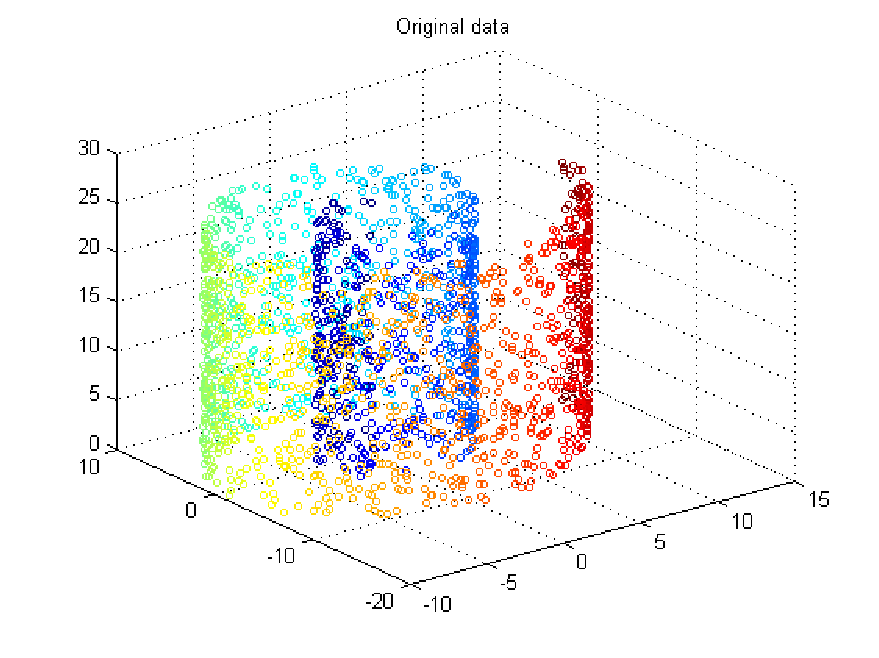
\includegraphics[height=0.25\textheight]{fig02/diffmap1.pdf}}
    \label{fig:1}
\end{minipage}
\vspace{2.0cm}
\begin{minipage}{7.0cm}
    \centering
    \subtop[]{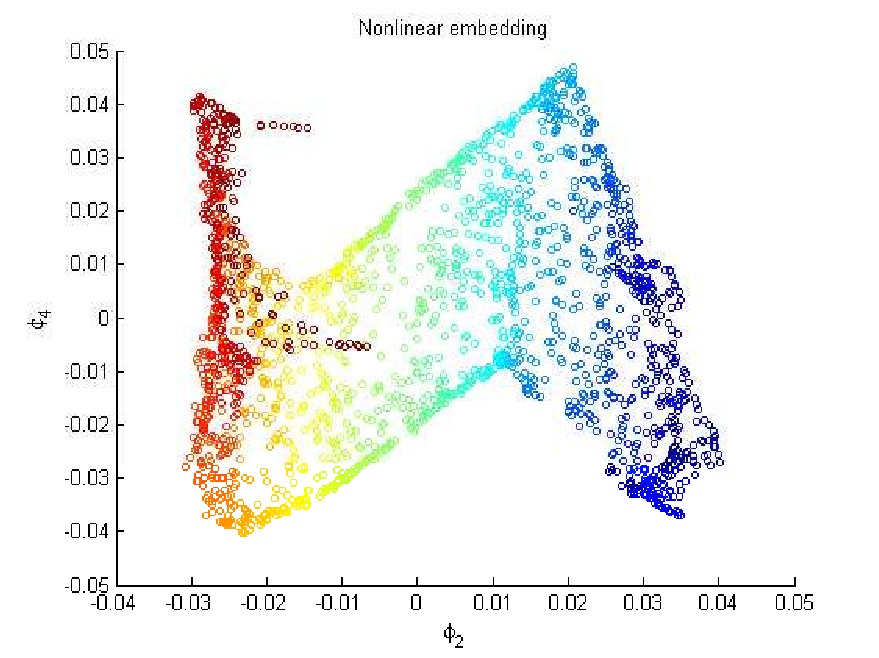
\includegraphics[height=0.25\textheight]{fig02/diffmap2.pdf}}
    \label{fig:2}
\end{minipage}
\mycaption[ALLData] {(a) Original example data 
(b) Non-linear embedding}
\end{figure}


\subsection{Locally Linear Embedding (LLE)}
In LLE a data manifold is constructed by finding a set of the nearest neighbours for each point\cite{Roweis2000}. Together they are used to compute a set of weights that describes each point as a linear combination of its neighbours. Finally, it uses an eigenvector-based technique to find the low-dimensional embedding of points, such that each point is still described with the same linear combination of its neighbours. Furthermore, the preservation of local properties allows for successful embedding of non convex manifolds.
{\bf LLE tends to handle non-uniform sample densities poorly because there is no fixed unit to prevent the weights from drifting as various regions differ in sample densities.}

\subsection{Laplacian Eigenmaps}
Laplacian Eigenmaps find a low-dimensional data representation by preserving local properties of the manifold.\cite{Belkin2003} Similar to LLE, a graph is built from neighbourhood information, with the distance between a point and it's K nearest neighbour is minimised. A weighting system is used such that in the low-dimensionality space the distance from a point to it's nearest neighbour is more significant to the cost function than other nearby points. {\bf put simply the closer a neighbour is to the selected data point the heavier its weighting.} The goal overall is to minimise the cost function based on the graph information to ensure that points close together in the high dimensionality data remain so after the reduction, preserving local distances. 


\subsection{Local Tangent Space Alignment (LTSA)}
LTSA is based on the intuition that when a manifold is correctly unfolded, all of the tangent hyperplanes to the manifold will become aligned.\cite{Zhang2003} In other words there will exist a linear mapping from high dimensionality data to a local tangent space which will have a linear mapping to a low-dimensionality data point. It begins by computing the k-nearest neighbours of every point. It computes the tangent space at every point by computing the d-first principal components in each local neighbourhood. It then optimizes to find an embedding that aligns the tangent spaces.


\subsection{Curvilinear Component Analysis (CCA)}
CCA is an learning algorithm that starts with larger distances before iterating to smaller ones.\cite{Demartines1997} It looks to output a configuration of points that preserves the original distances as much as possible while focusing on the smaller distances.

The large distance information will be overwritten by the smaller distance information unless a conflict occurs. The stress function of CCA is related to the sum of Bregman divergences which aim to generalise squared euclidean distances so they all share the same properties. If compromises between the larger and smaller distance information but be made the stress function determines this.

\section{Segmentation Methods}
Automatic segmentation is a crucial step in this project since on a larger scale much greater data sets will need to be used and collated from multiple sources. If these can be processed and automatically segmented this will remove any manual work required and make this a truly useful system. I will look at several methods that might aid me in finding meaningful characteristics to separate each punch.

\subsection{Dynamic Time Warping (DTW)}
Dynamic time warping is a time series comparison method that takes two temporal sequences, often which vary in time or speed and tries to calculate an optimal match. The two sequences are aligned and a similarity score is produced. This technique can be used on any data that can be represented in a linear fashion and has been successfully applied to fields such as signature recognition, voice recognition, partial shape matching and gait analysis. For example in gait analysis, similarities could be detected in the walking pattern of two people even though their speed and acceleration may be difference.
If a punch sequence is similar enough to others of the same type and different enough from other types of punch this could prove a useful method of recognising the start and end of a punch as well as the type of punch.

\begin{figure}[h]
    \centering
    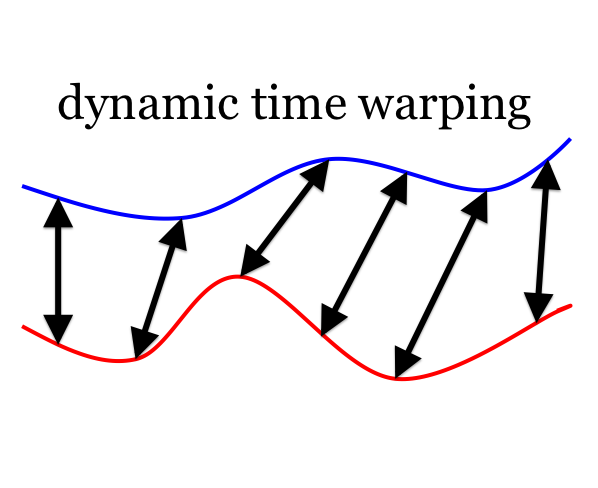
\includegraphics[height=0.25\textheight]{fig02/dtw}
    \mycaption[Kinect Device]{Dynamic time Warping}
    \label{fig:kinect}
\end{figure}


\subsection{Fourier Transformation (FT)}
The Fourier Transform is a mathematical transformation that can decompose a time series from the {\bf spatial domain (normal image space) | should this be time domain?} and transform it into the frequency domain. Any wave-like functions can be represented as a combination of simple sine waves by breaking down the original series into the sum of a set of oscillation functions, sines and cosines. The series is split into a magnitude spectrum which will comprise of complex exponentials and a phase spectrum which will encode angles in radians. 
The Fourier series of a function $f(x)$ is given by:
$$f(x)=\frac{1}{2}a_0 + \sum_{n=1}^\infty a_n cos(nx) + \sum_{n=1}^\infty b_n sin(nx)$$
Where:
$$a_0 = \frac{1}{\pi}\int_{-\infty}^\infty f(x)dx$$
$$a_n = \frac{1}{\pi}\int_{-\infty}^\infty f(x)cos(nx)dx$$
$$a_n = \frac{1}{\pi}\int_{-\infty}^\infty f(x)sin(nx)dx$$

Here the cosine coefficient is $a_n$ and the sine coefficient is $b_n$.

A property worth noting is that a shift in the time domain corresponds to a linear change in phase but does not alter the magnitude spectrum. Since my punches sequences over time are a continuous sinusoidal-like function I can use the discrete-time Fourier transform (DFTD) to obtain the Fourier coefficients which I hope will be unique enough to tell me something useful about the punch sequence.

\section{Classification Methods}

\subsection{Support Vector Machines}
A Support Vector Machine is a kernel-based method that is effective for highly dimensional datasets. The SVM uses a kernel to calculate the scalar product of two feature vectors in a high dimensional feature space. The decision function uses the hyper-planes, defined by the Support  vectors,  to  classify  the  data.  Only  significant  samples  are  taken  for  use  as support vectors so that a high variance will make less of a different to the accuracy of the model. \
\begin{figure}[h]
    \centering
    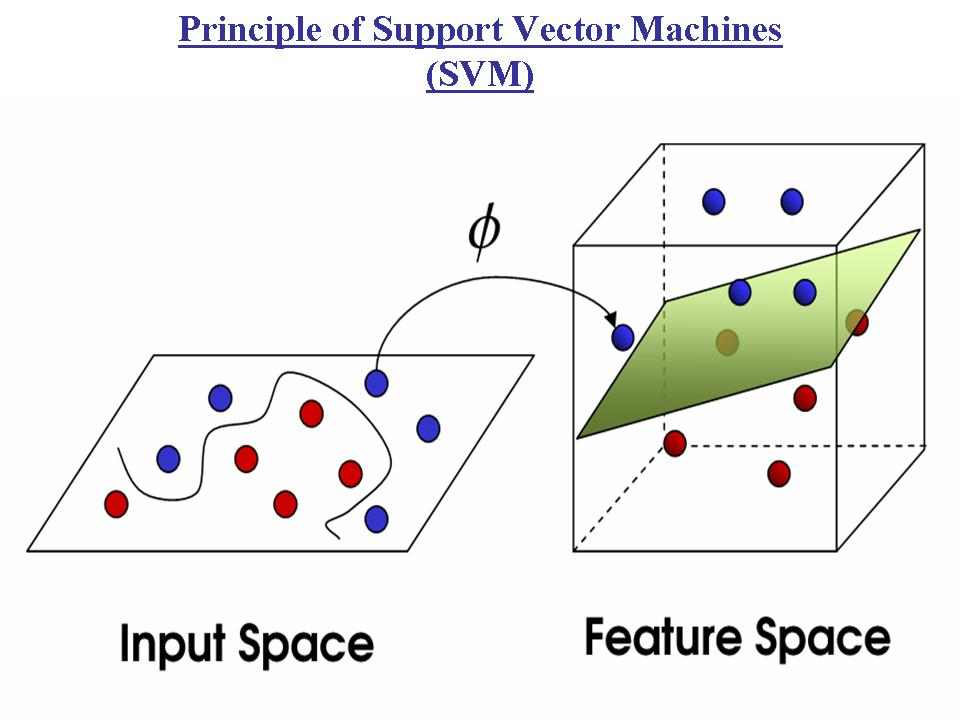
\includegraphics[height=0.25\textheight]{fig02/svm}
    \mycaption[Kinect Device]{Kinect Device.}
    \label{fig:kinect}
\end{figure}

\subsection{Neural Networks}
Neural networks are models based on the parallel processing of information similar to that of the brain. A NN can be configured for different applications such as clustering, pattern recognition, Dynamic Time series and curve fitting. They are able to derive meaning from complex data that human beings would be unable to notice and that other techniques will fail on. Crucially the networks are capable of approximating non-linear functions \textbf{unlike DTW. Neural networks learn by examples in the form of training data and are adaptive based on a system of weightings calculated by \% error. Other characteristics are their ability to self organise and the ability to work in real-time if sufficient parallelism is supported.}


Below is a model of a simple Neuron with many inputs and a single output. This is based on the biological models of a single neuron where a certain injection of current will decide if the neuron should fire. The `Integrate \& Fire' model is as follows:
$$C_m\frac{dv}{dt}=-G_l(V-E_l)+I_e$$
With time constraint: $$\tau_m = \frac{C_m}{G_l}$$
And membrane resistance: $$R_m = \frac{1}{G_l}$$
IF: $$V > V_th'$$ THEN: Generate a spike. $$V=V_reset$$

In this scenario the neuron has two modes of operation, testing and training. In the training mode the neuron can be trained to fire depending on a particular input pattern. In the testing mode when a recognised input pattern is detected the associated output from the training becomes the output. If the pattern is not recognised in the list of taught input patterns then it tries to identify that which is closest to it (which it does recognise) and produce an output matching that.
\begin{figure}[h]
    \centering
    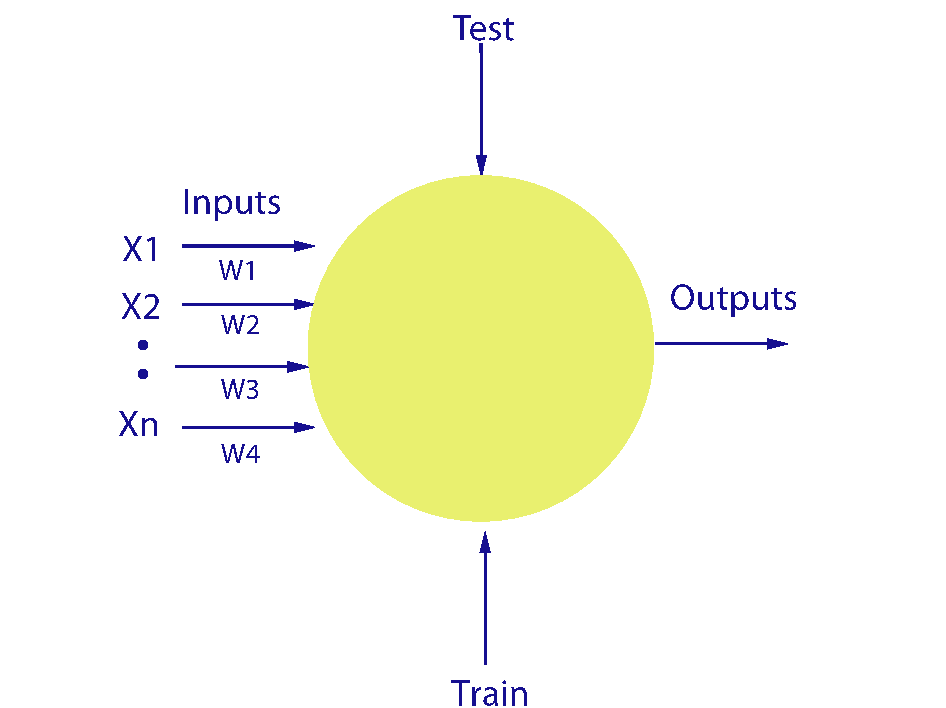
\includegraphics[height=0.25\textheight]{fig02/nnsimple.pdf}
    \mycaption[Kinect Device]{Kinect Device.}
    \label{fig:kinect}
\end{figure}


\paragraph{Back Propagation (BP)}
Neural networks (NN) work by connecting a series of single neurons into a learning network. Back Propagation is a learning algorithm whereby the network behaves similarly to above but with the added complexity that each input is given a weighting. This weighting is calculated iteratively by working out the error for each neuron like so: $Error_a = Ouput_a(1-Output_a)(Target_a - Output_a)$ which put simply is the difference between the correct output and the actual output for neuron A.

Since BP networks learn by example they must be given labelled training data which is used to correctly calculate the weights given to each input to give the required output. Since BPNN are ideal for pattern recognition and mapping tasks it could be suitable for use on punch sequences.

\begin{figure}[h]
    \centering
    \includegraphics[height=0.25\textheight]{fig02/nn.pdf}
    \mycaption[Kinect Device]{Kinect Device.}
    \label{fig:kinect}
\end{figure}


\subsection{Decision Trees \& Random Forest}
A predictive tree like model which maps observations about an object to reach a conclusion about its target value. In this model the `leaves' represent class labels while the branches themselves represent conjunctions of features that will lead to the class labels. Put simply each condition in an internal node while each outcome is an external node. Information gain is the difference between the initial entropy and the new entropy after following a branch along the decision tree. Since the goal of any machine learning technique is to achieve a low value of entropy to make accurate predictions, the decision tree is constructed such that each branch has the maximum possible information gain. The data is split by each feature that has the maximum information gain recursively for each branch.

Bagging is a method of assigning a measure of accuracy to sample estimates. We sample from an approximating distribution and try to approximately calculate the
properties of the estimator based on this. We measure a statistic from a sample of the population and then use this to say something about the whole population. For example, we might say that for our set of data a subset is used to determine a class. If any sample in the entire population follows the same tree rules then it will be labelled as in that class. We have used bootstrapped samples in our classifiers as they have been constructed using random sampling with replacement. 
This method is designed to improve the accuracy of machine learning algorithms, helping to reduce variance and hence over fitting. 

Random forest is an averaging algorithm which produces a diverse set of classifiers by introducing randomness in the classifier construction. Each tree is built from a bootstrapped sample from the training set. During construction the node splits are chosen based on the best split among a random subset of features, not the best split among all the features. Due to the randomness of this algorithm we expect it to have a slight bias compared to other decision tree models, however due to the averaging we expect a lower variance.

These Ensemble methods combine the predictions of multiple trees to come to a consensus.


\begin{figure}[h]
    \centering
    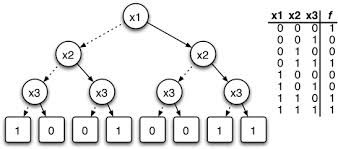
\includegraphics[height=0.25\textheight]{fig02/dtree}
    \mycaption[Kinect Device]{Kinect Device.}
    \label{fig:kinect}
\end{figure}


%=========================================================
\section{Punch Quality Algorithm}
I will be measuring quality in reference to a `ground truth' produced by a local professional. My aim is to create rules that are capable of detecting basic mistakes and provide feedback. I will start by targeting the characteristics as mentioned in the earlier background chapter, for example 
throwing a jab with the elbow sticking out instead of tucked is a classic beginners mistake.

